\documentclass[ngerman,oneside, a4letter]{article}
\usepackage[textwidth=16cm]{geometry}
\usepackage{graphicx}
\usepackage{hyperref}
\usepackage[utf8]{inputenc}
%\setcounter{chapter}{1}
\begin{document}

{\huge Installation von Pygame für das py2cd-Spieleframework}

\section{Vorbereitung}
Diese Anleitung ist beschreibt, wie man das für \emph{py2cd} benötigte \emph{pygame}-Framework (\url{http:pygame.org}) herunterlädt und installiert. Diese Anleitung ist nur für Windows 
\\
\\
\textbf{Hinweis:} Es wird vorausgesetzt, dass Python 3 bereits installiert ist und das Python und Pip zur Pfad-Umgebungsvariablen hinzugefügt worden sind.
\\
Falls nicht, kann eine Anleitung zur Installation von Python kann unter \url{https://github.com/coderdojoka/Materialien/blob/master/Installation/installation_python.pdf} gefunden werden.

\subsection{Download}
Zuerst muss \emph{pygame} installiert werden. Dafür ist es am Einfachsten, wenn man das vorkompilierte \emph{pygame}-Paket mit dem Namen: \emph{pygame-1.9.2a0-cp34-none-win32.whl} (cp34 $\rightarrow$ für Python 3.4) von der Seite \url{http://www.lfd.uci.edu/~gohlke/pythonlibs/#pygame} herunterlädt.
\\
\textbf{Hinweis:} Es dauert eine Weile bis die Seite lädt und an die richtige Stelle springt.

\begin{center}
	\makebox[\textwidth]{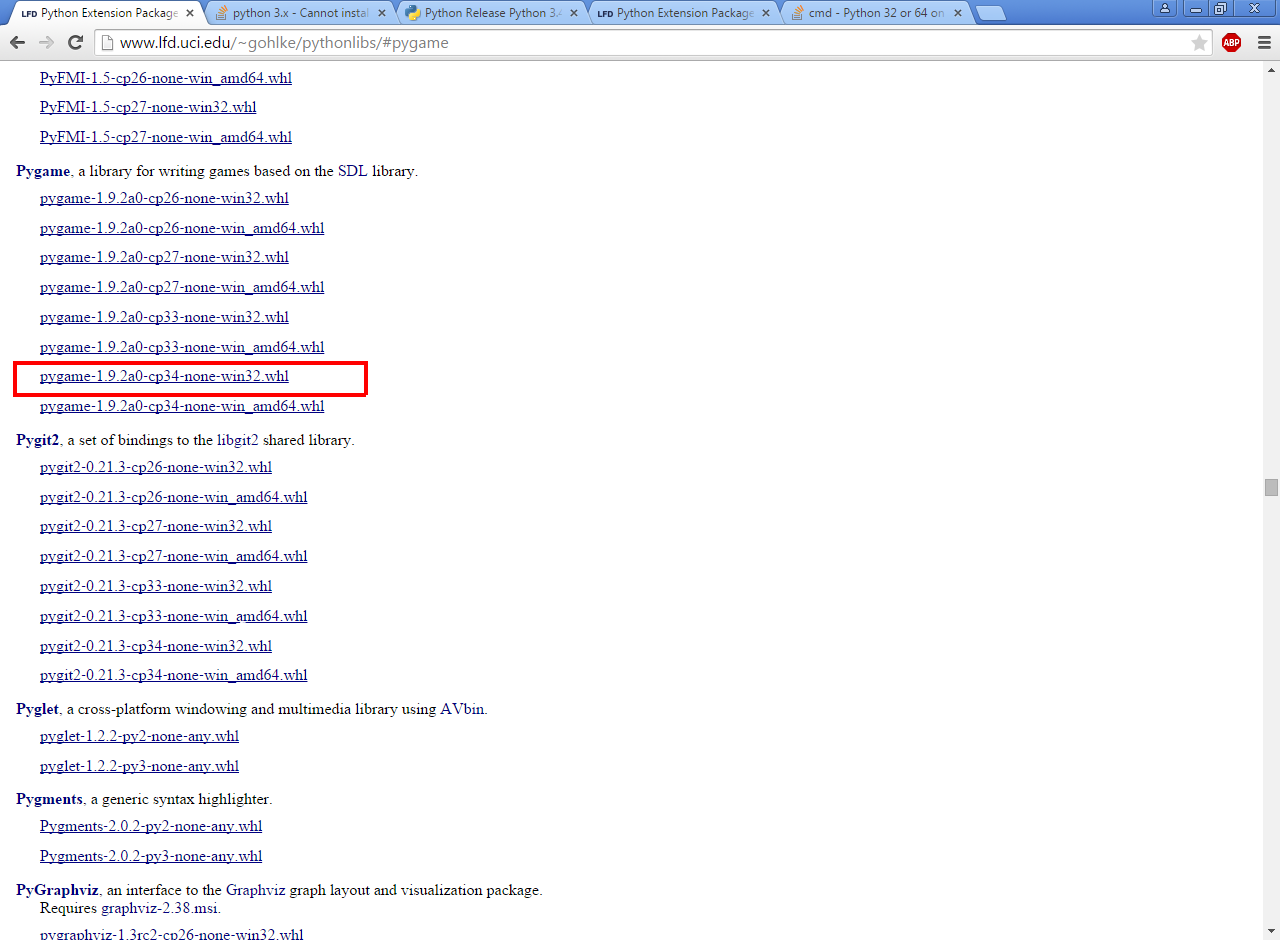
\includegraphics[width=.95\textwidth]{bilder/download_pygame}}
\end{center}

\section{Installation}
Um das heruntergeladene pygame-Paket zu installieren verwenden wir \emph{pip}.
Dazu öffnet man die Windowskommandozeile, z.B. durch Suchen nach 'cmd' im Windows-Suchfeld.

\begin{center}
	\makebox[\textwidth]{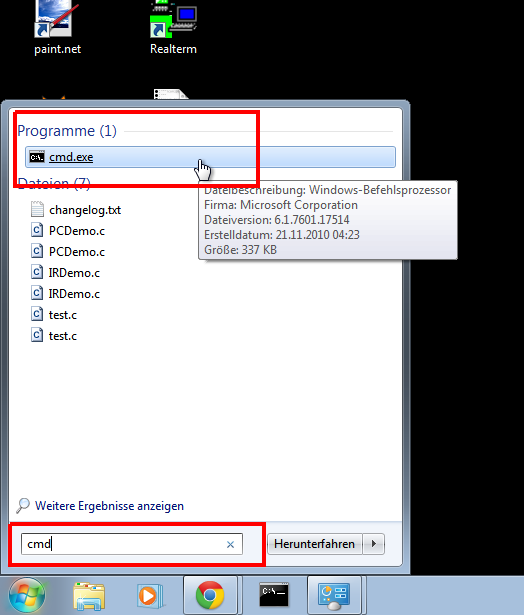
\includegraphics[width=.8\textwidth]{bilder/cmd}}
	\end{center}


\pagebreak

\noindent Um \emph{pygame} zu installieren müssen wir den Ort der heruntergeladen Datei kennen. Diese ist wahrscheinlich im \emph{Downloads}-Ordner des aktuellen Benutzers zu finden, z.B. unter:
\\
'C:\textbackslash users\textbackslash me\textbackslash Downloads\textbackslash pygame-1.9.2a0-cp34-none-win32.whl'
\\
\\
Die Windowskommandozeile startet standardmäßig im Benutzerverzeichnis (dies sieht man am linken Bildschirmrand auch in der Kommandozeile geschrieben) hier also:
\\
'C:\textbackslash users\textbackslash me\textbackslash'
\\
\\
Relativ zu diesem Pfad liegt also die Datei unter:
\\'Downloads\textbackslash pygame-1.9.2a0-cp34-none-win32.whl'. 
\\
\\
Nun wird der folgende Befehl in der Kommandozeile eingetippt:
\\
\emph{pip install -\,-use-wheel Downloads\textbackslash pygame-1.9.2a0-cp34-none-win32.whl}
\\
\\
\textbf{Hinweis:} Liegt die Datei in einem anderen Verzeichnis, muss der Pfad natürlich dementsprechend angepasst werden.
\\\textbf{Tip:} Hält man im Windows-Explorer die Shift-Taste gedrückt und Rechts-klickt auf den Ordner, so kann man im Menü den Eintrag: 'Kommandozeile hier öffnen' auswählen.

\begin{center}
	\makebox[\textwidth]{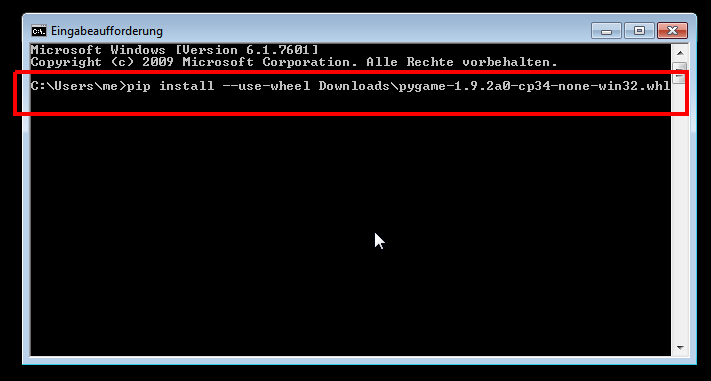
\includegraphics[width=\textwidth]{bilder/pip_install}}
\end{center}

\pagebreak
\noindent Hat alles geklappt, dann sollte eine folgende oder ähnliche Meldung in der Kommandozeile zu sehen sein:
\begin{center}
	\makebox[\textwidth]{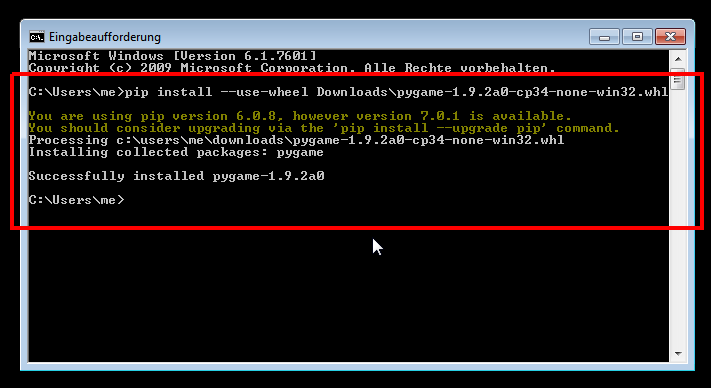
\includegraphics[width=\textwidth]{bilder/pip_install_done}}
\end{center}

\pagebreak
\section{Installation überprüfen}
Als letzen Schritt kann die Installation noch überprüft werden.
Dazu tippt man in der Windows-Kommandozeile folgende Befehle und bestätigt diese mit der Enter-Taste:
\\
\\
\begin{table}[h]
	\begin{tabular}{ll}

		\emph{python}        & startet die Python-Shell. Dort schreibt man dann:            \\ 
		\emph{import pygame} & um zu testen ob pygame geladen werden kann. Danach:                \\ 
		\emph{pygame}        & um Informationen  installierten \emph\{pygame\}-Paket zu erhalten. \\ 
	\end{tabular}
\end{table}
\\
\\
Das Ganze sollte dann in etwa so aussehen:
\begin{center}
	\makebox[\textwidth]{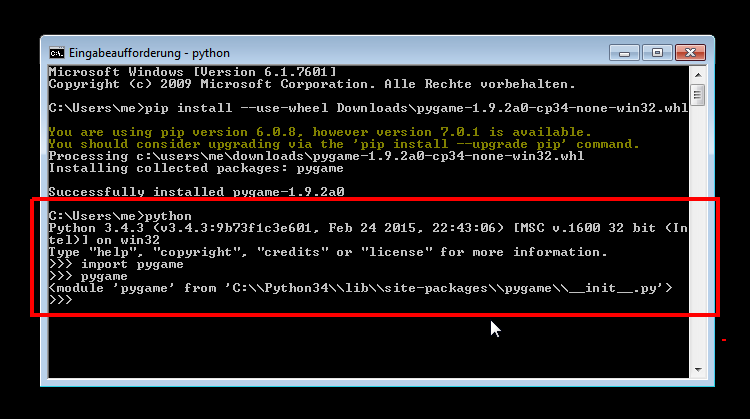
\includegraphics[width=\textwidth]{bilder/pip_install_check}}
\end{center}
Pygame ist jetzt erfolgreich installiert!

\section{Py2cd}
Um \emph{py2cd} benutzen zu können, lädt man sich am Besten die aktuellen Quelldateien via GitHub \url{https://github.com/coderdojoka/py2cd} herunter oder frägt den Mentor seines Vertrauens.
\end{document}